\chapter{Documento de Diseño del Juego (GDD)}
\label{GDD}

\section{Descripción general}
El juego que se pretende desarrollar se basa en el apartado de navegación por el mapa y combate
típicos en los \ac{RTS}. A lo largo de los distintos niveles, el jugador deberá hacer
frente a distintos desafios como pueden ser: escoltar con sus unidades de un punto
del mapa a otro a un personaje importante y/o eliminar a todas las entidades enemigas del escenario.

\section{Mecánicas}
Durante el juego podremos ejecutar una serie de ordenes sobre nuestras unidades para cambiar
su distribución, ordenarles que se desplazen y/o que ataquen a enemigos.\\
Para el desplazamiento por el mapa, el jugador contará con un marcador en el mapa el cual
será capaz de mover para que sus unidades lo sigan mientras les sea posible.

\begin{figure}[ht]
\centering
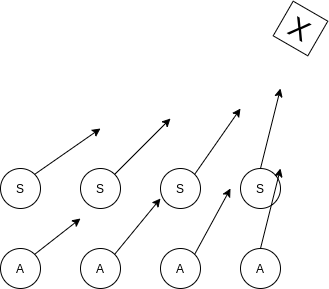
\includegraphics[width=0.35\textwidth]{imagenes/gdd/Following.png}
\caption{MockUp Seguimiento de la marca del jugador.}
\label{fig:mockup_following}
\end{figure}

En cuanto a las posibles formaciones para nuestras unidades, encontramos las siguientes:

\newpage

\begin{itemize}
\item \textbf{Sin formación:} las unidades no tendrán nigún paramétro de ordenación.

\begin{figure}[ht]
\centering
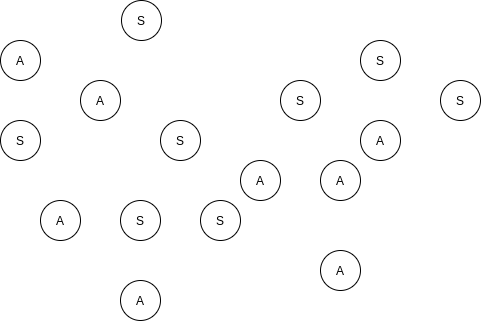
\includegraphics[width=0.32\textwidth]{imagenes/gdd/Formacion-desordenada.png}
\caption{MockUp unidades desordenada.}
\label{mockup_desordenada}
\end{figure}

\item \textbf{En anillo:} formación circular alrededor de una unidad especial. En caso de
no haber unidad escoltada el centro estará vacío. 
\end{itemize} 


\begin{figure}[ht]
\centering
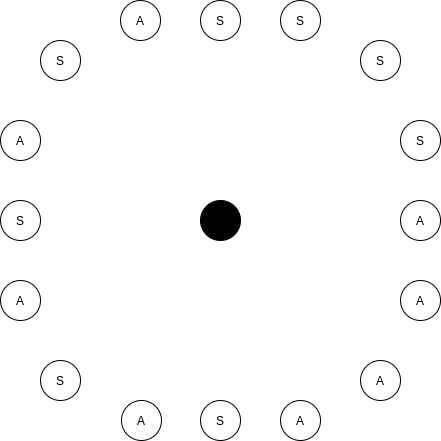
\includegraphics[width=0.32\textwidth]{imagenes/gdd/Formacion-anillo.png}
\caption{MockUp unidades en anillo.}
\label{mockup_anillo}
\end{figure}

Por último podemos ordenar a las unidades que mantengan una estrategia definida:

\begin{itemize}
\item \textbf{Huida:} en este modo las unidades seguirán el marcador sin pararse a pelear con unidades
cercanas enemigas.

\item \textbf{Agresivo:} en el momento en el que la tropa divisa un enemigo saldrá diracto a atacarle,
aunque se aleje esta le seguirá mientras siga en su rango de detección.
\end{itemize} 

Aunque el jugador marque una estrategia y forma de plantear el combate, las unidades podrán
decidir si seguir al jugador o revelarse. Si los soldados cercanos están siendo masacrados
existe la posibilidad de que tengan miedo y huyan, si las unidades enemigas nos superan en número
la unidad puede decidir si permanecer en defensa en lugar de atacar de forma activa.

\section{Unidades}
Entre las unidades podemos encontrar dos arquetipos con carácteristicas propias
que nos permitiran crear variedad en las soluciones a la hora de superar el
nivel.

Los tipos son los siguientes:
\begin{itemize}
	\item \textbf{Soldado:} es la unidad más básica que podemos encontrar en el campo de
							guerra, esta armado con una espada y posee estadisticas
							bajas.
	\item \textbf{Arquero:} va equipado con arco y flechas para atacar a distancia a
							sus rivales, tiene menos resistencia que los soldados por
							lo que tendremos que protegerlos para asegurar su
							supervivencia.
\end{itemize}

\begin{table}[ht]
\begin{center}
\begin{tabular}{|c|c|c|c|c|}
\hline
        & Daño & Vida  & Rango  & Tiempo de ataque \\ 
\hline
\hline
Soldado & 7    & 24    & Melee & 2 seg.\\ 
\hline
Arquero & 4    & 14    & Largo & 3 seg.\\ 
\hline
\end{tabular}
\caption{Unidades y estadísticas}
\end{center}
\end{table}

\section{Controles}
A la hora de jugar tendremos una serie de teclas asignadas a las acciones que el
jugador puede realizar cuando interactúe con el juego. Para enumerarlas dividiremos las
acciones en dos grupos, dependiendo de si son para navegar por los menús o si
representan acciones durante el \textit{gameplay}.

Para avanzar por los menús usaremos la tecla \textbf{Enter} una vez estemos sobre la opción deseada o
para avanzar los mensajes explicativos del tutorial/informativos.

Las asignadas para jugar son las siguientes:
\begin{itemize}
	\item \textbf{Flechas o W/A/S/D:} mediante estas teclas podremos desplazar el puntero por el mapa.
	\item \textbf{Barra Espaciadora:} con esta otra podremos ordenar atacar a nuestras unidades,
									  si no encuentran una unidades enemiga en su rango se mantendrá
									  en seguimiento del puntero.
	\item \textbf{Ctrl:} activa el modo huída y las unidades dejarán de combatir y seguirán el
					  puntero.	
	\item \textbf{Z:} activa la formación en anillo.									  
	\item \textbf{X:} desactiva toda formación.
	\item \textbf{Ratón:} interactuar con el \textit{HUD}.
\end{itemize}

Tanto la \textbf{formación} como el \textbf{comportamiento} de las unidades se podrá cambiar desde un
pequeño \textbf{\textit{HUD}},que se encuentra en la esquina inferior izquierda.

\section{Pantallas}
Al ejecutar el programa la primera pantalla que aparecerá será la de 
inicio. Se compone del título del juego, la fecha de lanzamiento,
el nombre del desarrollador y un mensaje que nos indica que tenemos que pulsar al tecla
\textit{entre} para continuar, esta pantalla se mantendrá hasta que el jugador presione
dicha tecla.\\
Una vez pulsado el botón indicado se procederá a cargar el juego mientras se muestra
una barra que indica el progreso de cargado.

\begin{figure}[h]
\centering
\begin{minipage}[c]{0.42\linewidth}
	\hspace{9mm}
	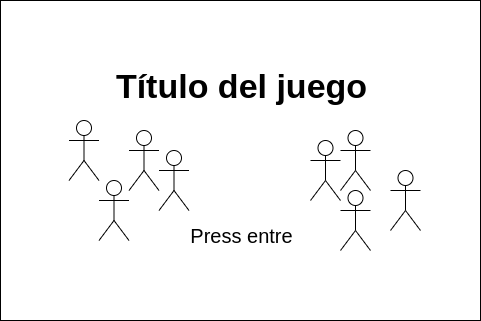
\includegraphics[width=0.7\textwidth]{imagenes/gdd/pantallas/Pantalla_ini.png}
	\caption{MockUp inicio.}
	\label{mockup_ini}
\end{minipage}
\begin{minipage}[c]{0.42\linewidth}
	\hspace{9mm}
	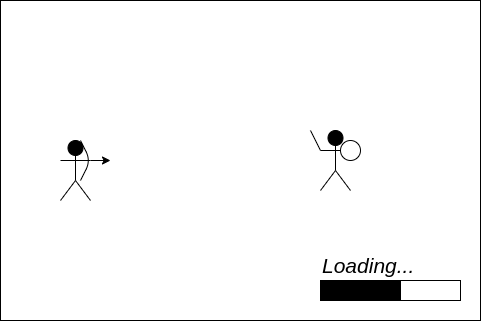
\includegraphics[width=0.7\textwidth]{imagenes/gdd/pantallas/Pantalla_carga.png}
	\caption{MockUp carga.}
	\label{mockup_carga}
\end{minipage}	
\end{figure}

A continuación de la carga pasaremos directamente al escenario, donde se desarrollará el
\textit{gameplay} y nos mantendremos en esta pantalla hasta que termine el juego, ya sea
por victoria o derrota del jugador.

\begin{figure}[ht]
\centering
\begin{minipage}[c]{0.45\linewidth}
	\hspace{9mm}
	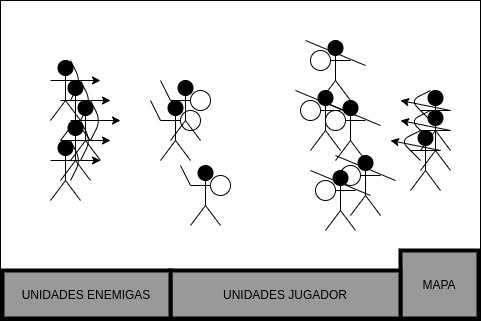
\includegraphics[width=0.7\textwidth]{imagenes/gdd/pantallas/Pantalla_gameplay.png}
	\caption{MockUp juego.}
	\label{mockup_juego}
\end{minipage}
\begin{minipage}[c]{0.45\linewidth}
	\hspace{9mm}
	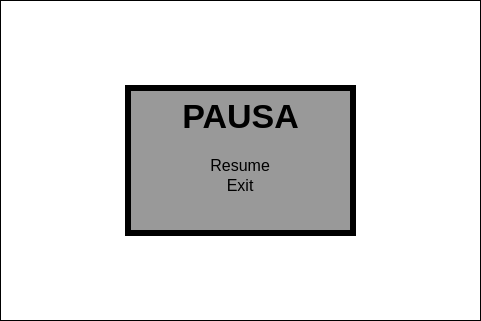
\includegraphics[width=0.7\textwidth]{imagenes/gdd/pantallas/Pantalla_pausa.png}
	\caption{MockUp pausa.}
	\label{mockup_pausa}
\end{minipage}	
\end{figure}

El final de la partida nos trae dos posibles escenarios, la victoria y la derrota. 
Para cada uno saldrá su respectivo mensaje y pasado un momento se nos mandará automáticamente a 
la pantalla de inicio.

Como última pantalla con la que el jugador podrá interactuar es la del menú de
pausa, en el cual se le dará la opción de salir o de volver a la
partida, mientras esta pantalla este activa la acción en el juego se paralizará hasta
que el jugador decida. 

\begin{figure}[ht]
\centering
\begin{minipage}[c]{0.45\linewidth}
	\hspace{9mm}
	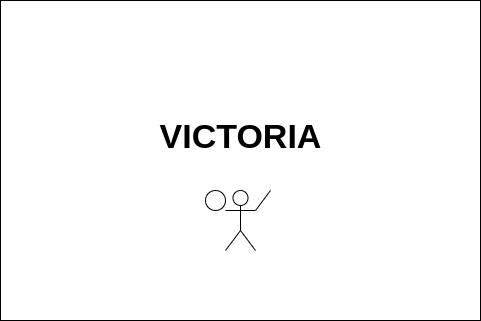
\includegraphics[width=0.7\textwidth]{imagenes/gdd/pantallas/Pantalla_victoria.png}
	\caption{MockUp victoria.}
	\label{mockup_victoria}
\end{minipage}
\begin{minipage}[c]{0.45\linewidth}
	\hspace{9mm}
	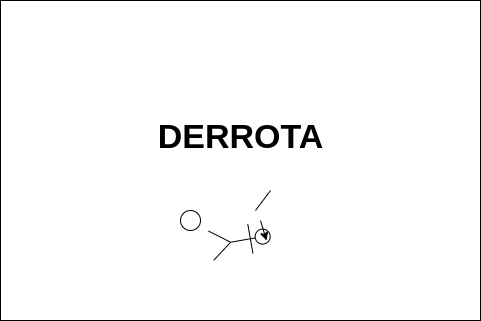
\includegraphics[width=0.7\textwidth]{imagenes/gdd/pantallas/Pantalla_derrota.png}
	\caption{MockUp derrota.}
	\label{mockup_derrota}
\end{minipage}	
\end{figure}

\section{Estados del juego}
Una vez mostradas todas las posibles pantallas con las que podrá interactuar el jugador,
es interesante dibujar un diagrama de flujo que plasme sus conexiones y posibilidades
con el fin de crear una representación gráfica que sirva como esquema global.

Dicho esquema podemos encontrarlo en la figura siguiente:

\begin{figure}[ht]
\centering
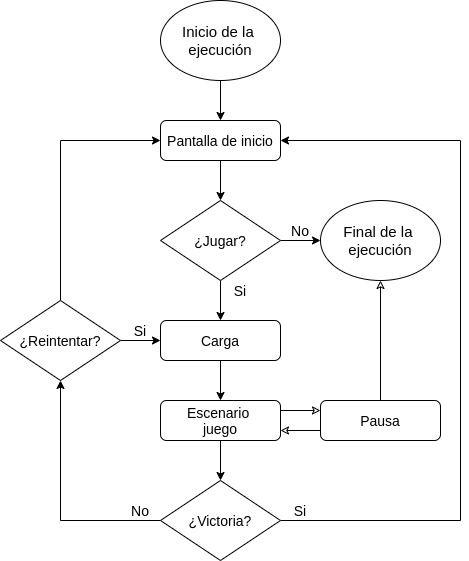
\includegraphics[width=0.45\textwidth]{imagenes/gdd/pantallas/flow_ejecucion.png}
\caption{MockUp flujo de ejecución.}
\label{esq:flow_juego}
\end{figure}

\section{Niveles}
El juego contiene actualmente 2 niveles, el primero se trata de un nivel introductorio
en el que encontraremos grupos pequeños de unidades que será fáciles de abatir para que el jugador experimente
como es el combate en el juego, además, a lo largo del nivel queremos poner marcadores para dar indicaciones
al jugador de como jugar o \textit{tips} para superar los niveles de forma satisfactoria.
El nivel se supera matando a los enemigos.

\begin{figure}[ht]
\centering
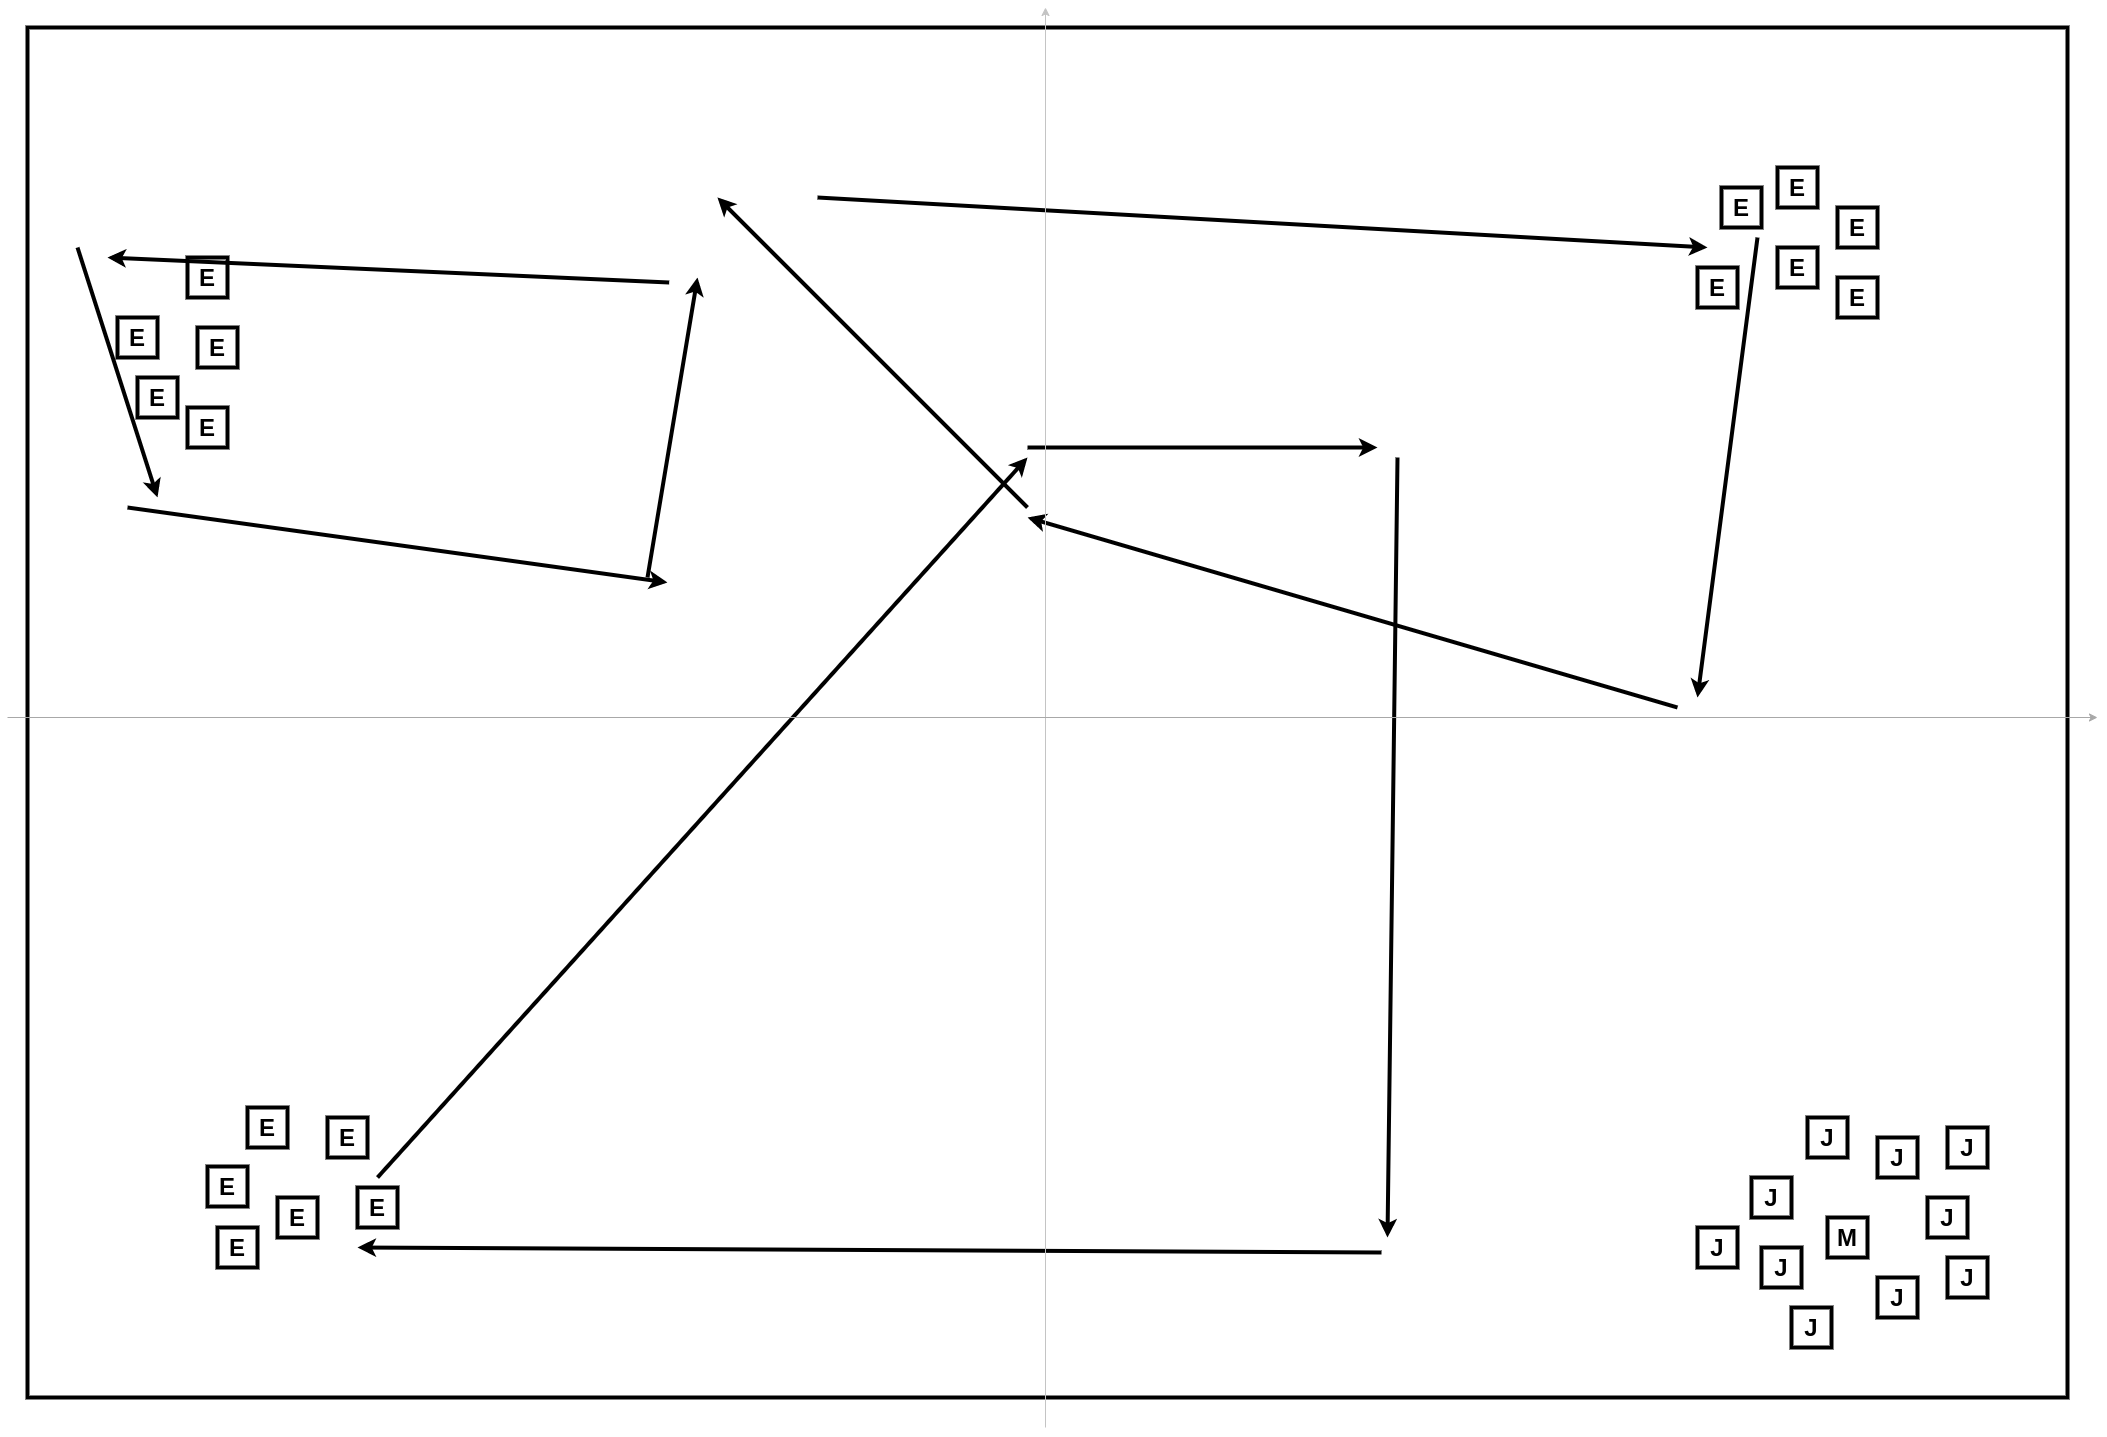
\includegraphics[width=0.6\textwidth]{imagenes/gdd/nivel0.png}
\caption{MockUp nivel 0.}
\label{esq:lvl0}
\end{figure}

En el segundo nivel se muestra otro de los objetivos posibles en el juego, el cual se trata de alcanzar
una zona de huida/meta más allá de las tropas enemigas, en este nivel encontraremos
grupos más grandes de enemigos que nos pueden vencer y hacernos repetir el nivel, por ello podremos optar
por intentar derrotarlos o buscar una ruta que nos evite el conflicto lo máximo posible. 

\begin{figure}[ht]
\centering
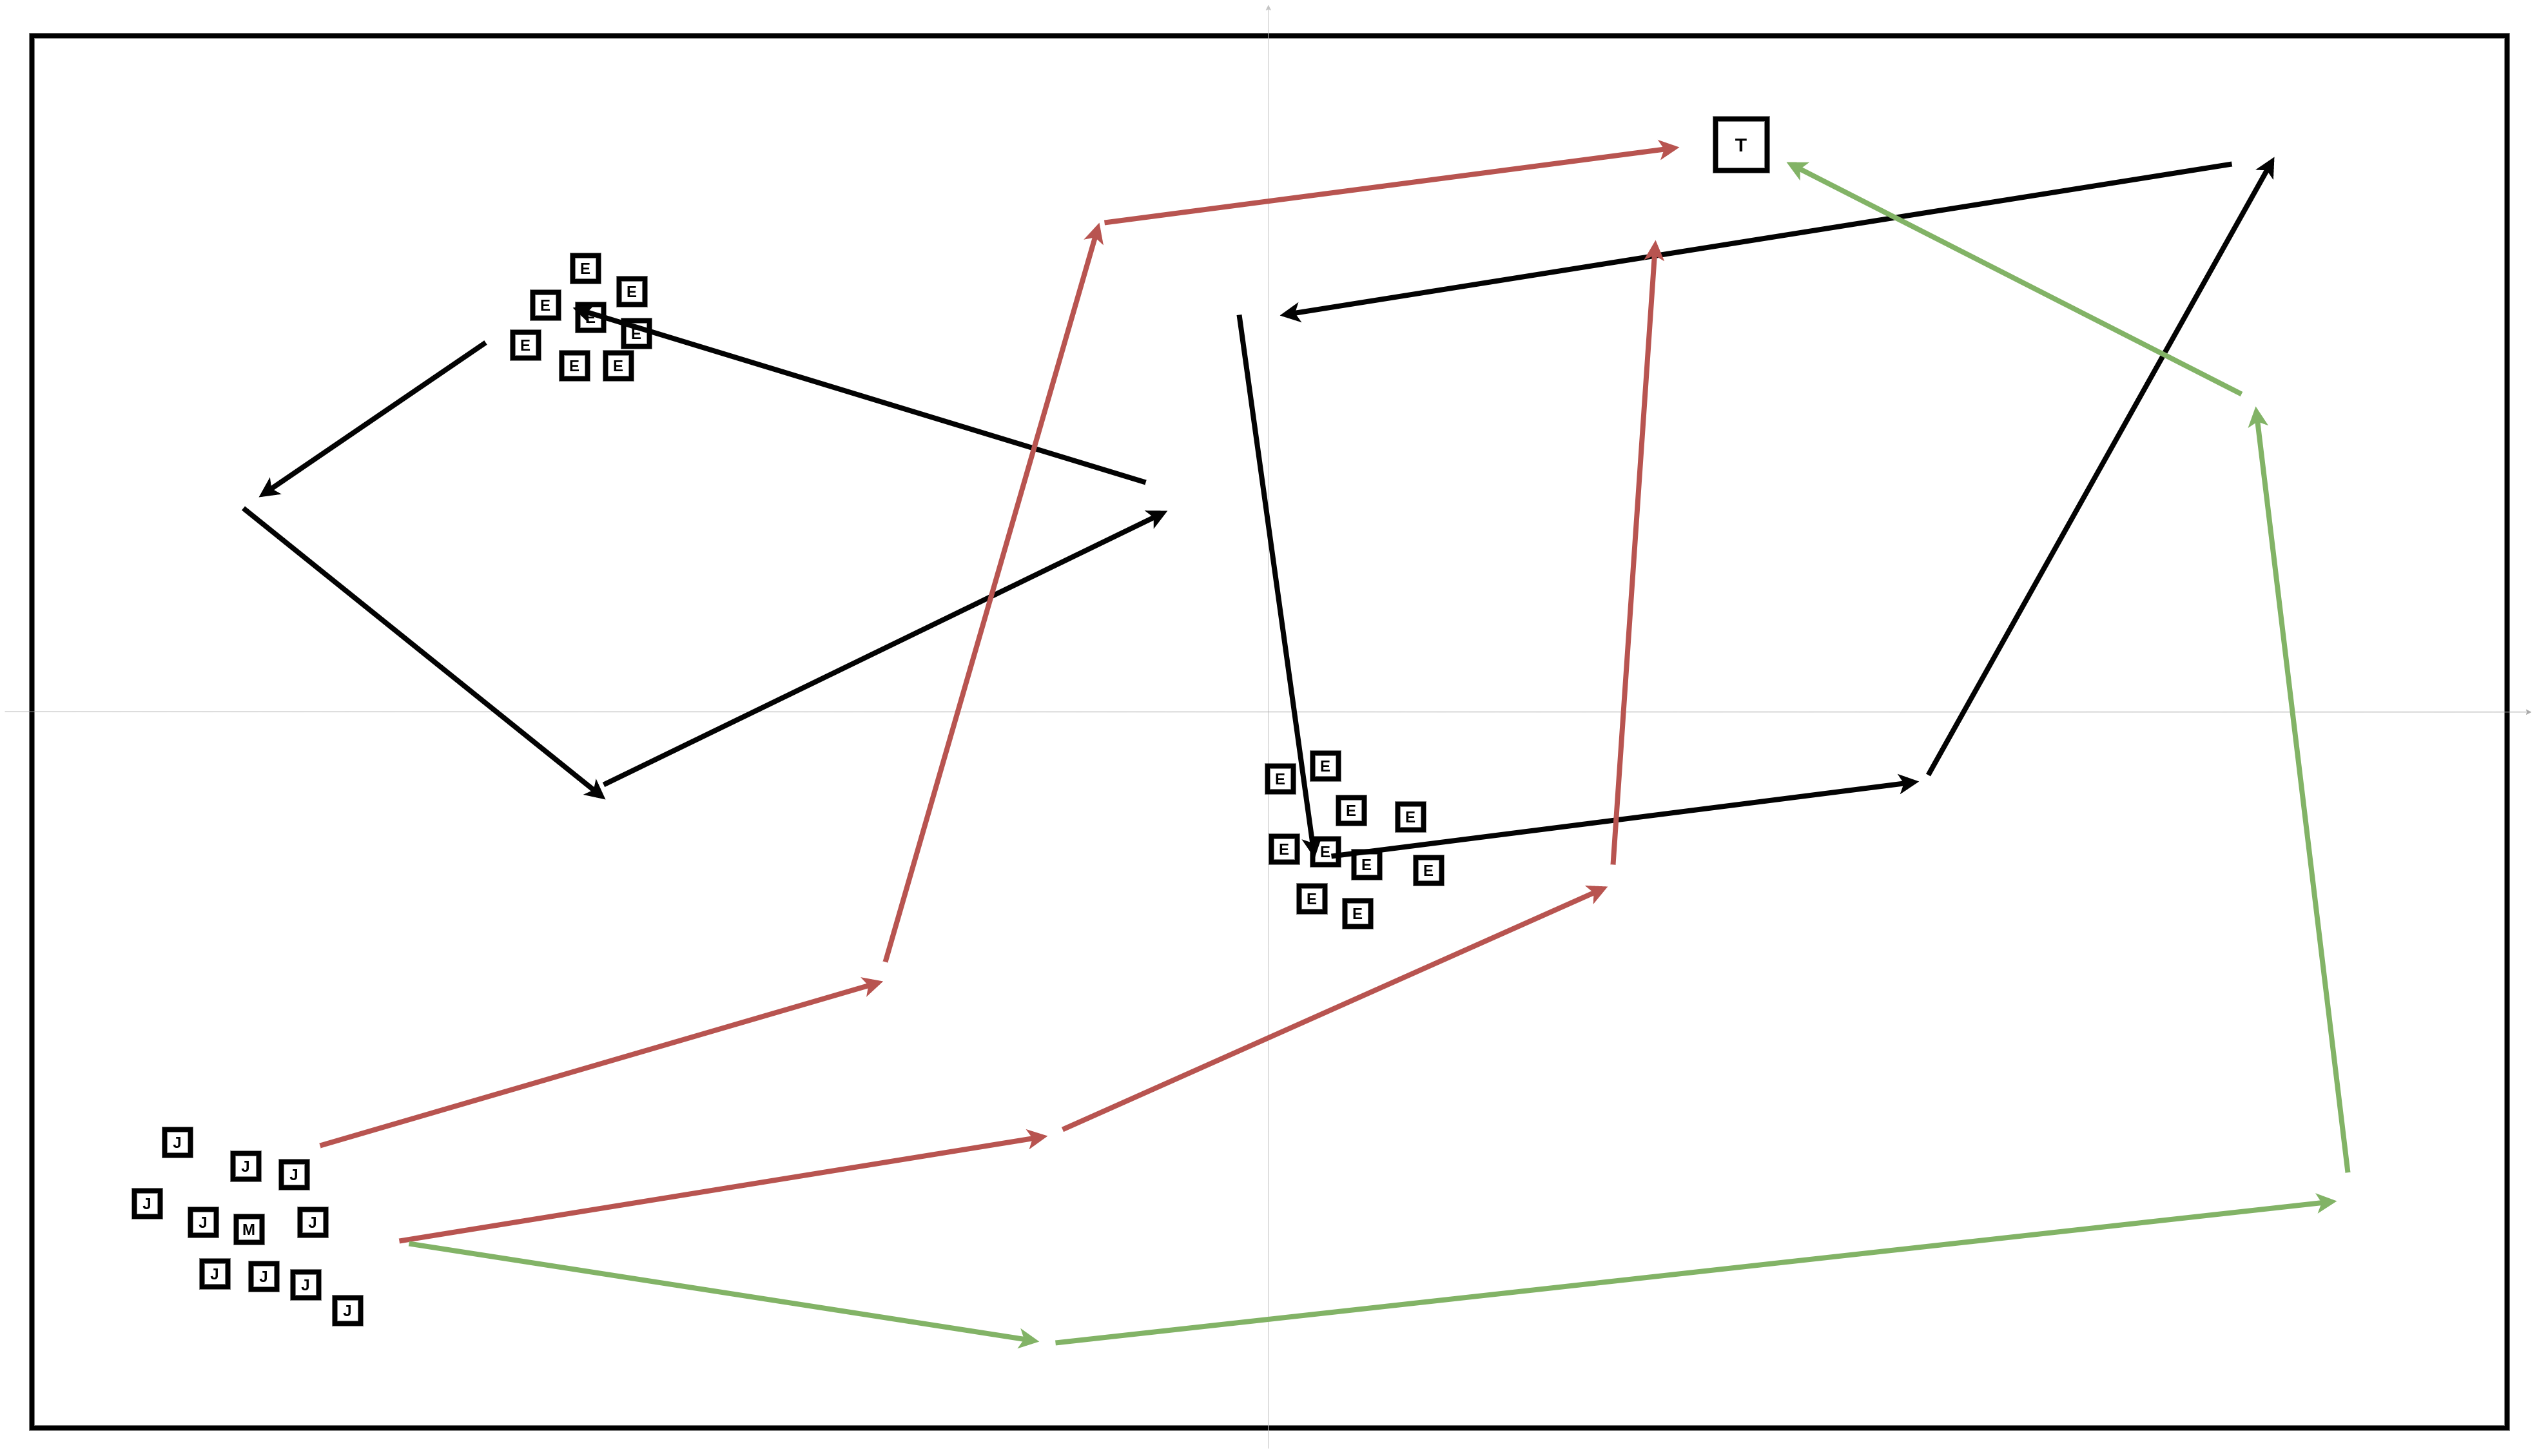
\includegraphics[width=0.6\textwidth]{imagenes/gdd/nivel1.png}
\caption{MockUp nivel 1.}
\label{esq:lvl1}
\end{figure}

\section{Escenarios}
A lo largo de los niveles la intención es que nos encontremos con distintos biomas como
pueden ser praderas, bosque o desiertos como los que podemos encontrar en \ac{AoE} II.

\begin{figure}[ht]
\centering
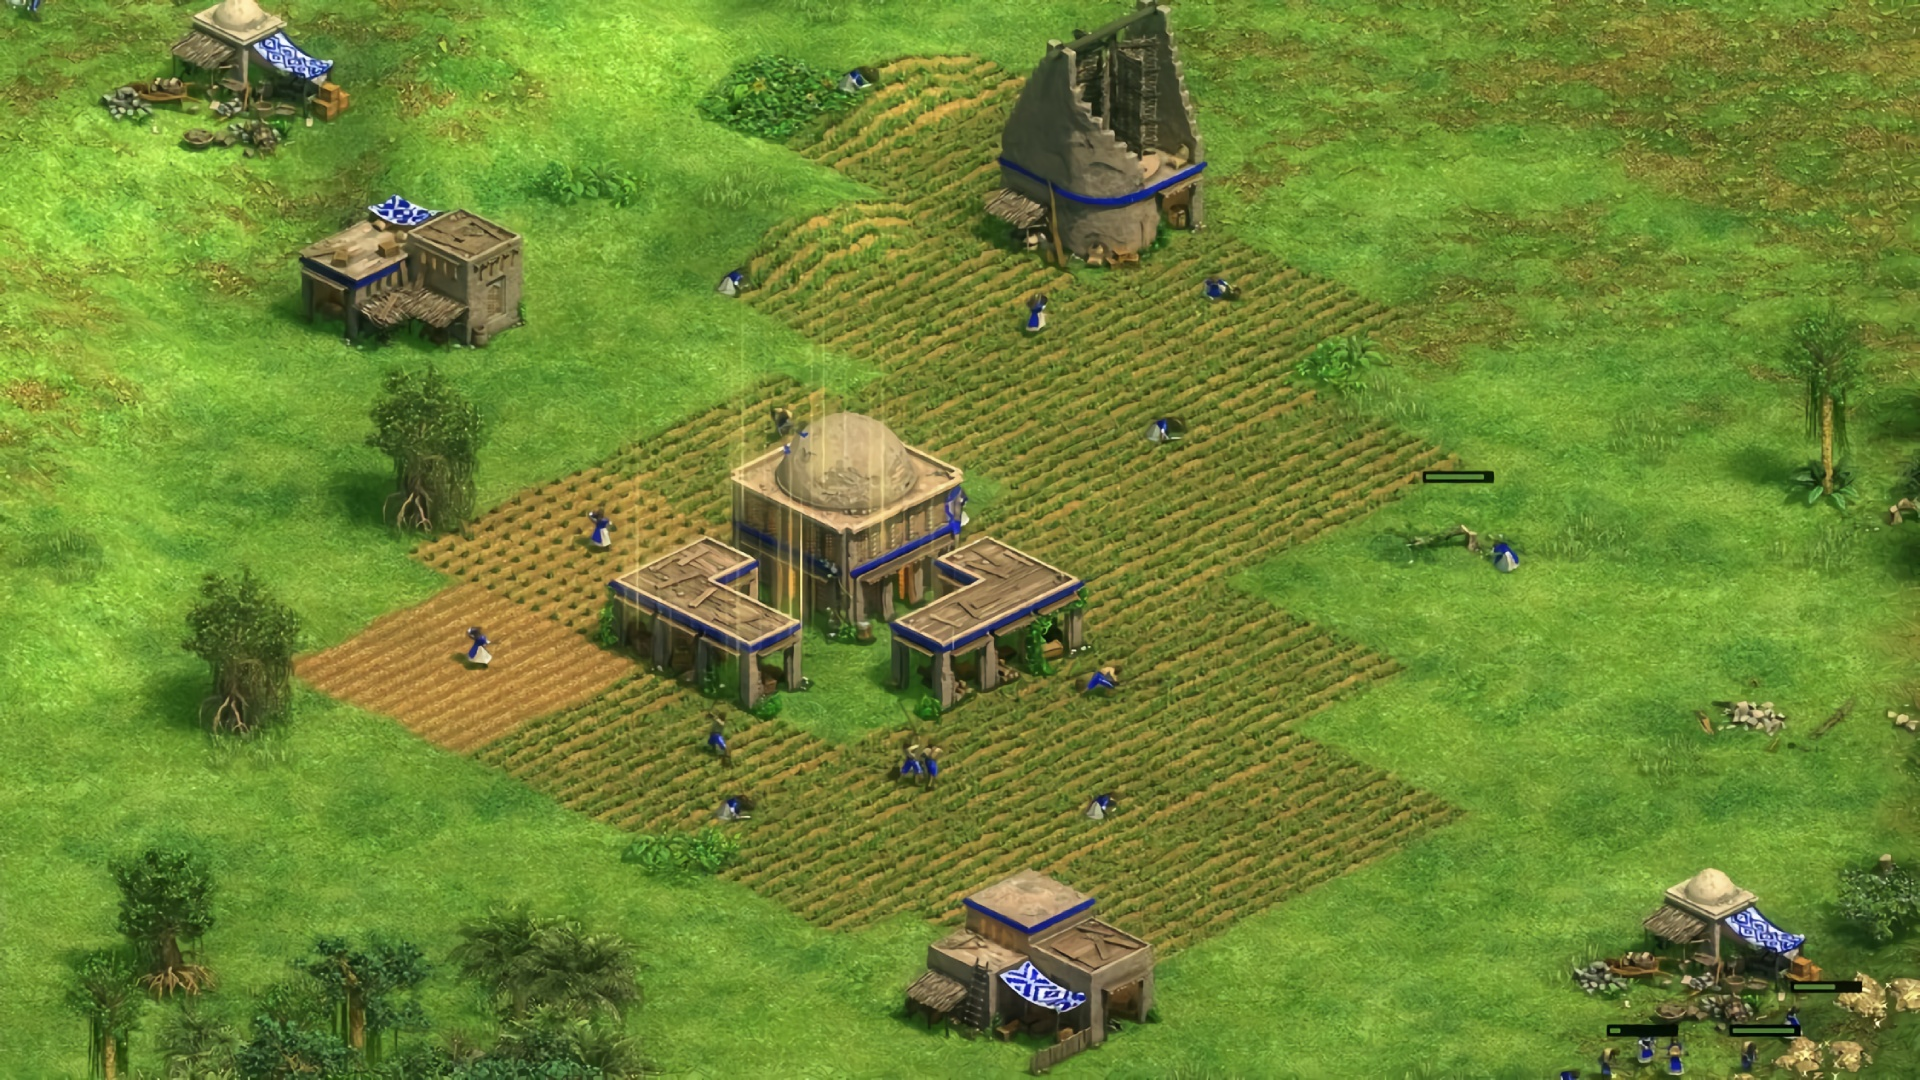
\includegraphics[width=0.6\textwidth]{imagenes/gdd/mapa_aoe_1.jpg}
\caption{Ejemplo escenario con vegetación.}
\label{img:mapa_aoe1}
\end{figure}

Además de imitar el estilo artístico el juego se desarrollará empleando una cámara
aerea fija manteniendo una perspectiva isométrica que nos permitirá visualizar desde
un punto elevado una gran porción del escenario, esto lo haremos con el fin de dar al
jugador la posibilidad de conocer lo máximo posible el territorio cercano posible y a la
vez le libramos de tener que estar preocuparse de situar la cámara para cada momento. \\
Al mantener una posición fija podemos situar todos los elementos en la escena de forma
que no obstaculicen la visión o molesten al jugador.

En las primeras versiones del proyecto el juego todos los elementos serán 2D y la vista será
un plano picado, el final deseable será poder pasar a un entorno 3D.

\section{Sistema de cámaras}
Si quisieramos mostrar todo el nivel por pantalla, tendríamos el problema de que los elementos
quedarían dibujados con un tamaño demasiado pequeño si el nivel supera las dimensiones de la pantalla,
por ello, si queremos poder diseñar niveles con las dimensiones que queramos deberemos mostrar únicamente
las fracción del nivel que ocupamos en cada momento.

Por lo que, tendremos una cámara la cual seguirá al puntero del jugador por el nivel y tendremos el
minimapa para poder ubicarnos en el nivel.

\section{Mínimo producto viable}
Una vez planteadas todas las características deseadas para el videojuego, es acosenjable
decidir que partes del producto son vitales para mostrar la experiencia
de juego deseable, el hecho de marcar estos objetivos nos ayudará a poder desarrollar una
versión reducida del proyecto que nos permita dar la sensación de tener un producto acabado.\\
Es importante realizar este proceso ya que por motivos internos o externos al equipo de desarrollo,
siempre existen contratiempos que nos impidan conseguir todos los objetivos propuestos en el
documento.

En cuanto a las etapas en la ejecución del juego, encontramos esencial el poder finalizar el nivel,
ya sea por victoria o derrota. Acto seguido volver al comienzo del nivel, dejando a un lado un
posible menú inicial y de pausa.

Una vez en partida el juego constará de un nivel único compuesto por: un escenario estático
mínimo, un conjunto de unidades propiedad del jugador y otro perteneciente a la máquina.\\
Al inicio del juego el jugador se encontrará quieto en uno de los extremos del nivel y el enemigo 
estará patrullando por una zona designada, dejando así a elección del jugador la distribución y el
momento exacto en el que comenzará la disputa.

En lo referente a las mecánicas y jugabilidad, es importante que el jugador sea capaz de poder
mover a sus unidades por el escenario y ordenarles atacar, por otro lado sería deseable poder
ajustar algunos parámetros del comportamiento de su ejercito para poder pasar el nivel de más
de una forma.\\
Otro lado la \ac{IA} debe ser capaz de detectar el acercamiento del jugador y responder a la
ofensiva, dejando la capacidad de tomar la iniciativa y variar su estrategia para versiones
más completas. Ambos ejercitos se compondrán de soldados y arqueros.

En lo referente al apartado visual, sería deseable tener sprites para unidades y escenario pero
de ser necesario podemos mantener el sistema de \textit{render} inicial.


\section{Actualización: 13/04/21}
\begin{itemize}
	\item Corregido el movimiento lento de las entidades en algunos momentos cuando estaban en el radio
	de frenada, era debido a un cálculo erróneo en las diviones con el tipo de dato en coma fija.
	
	\item Creació de una componente para las colisiones y integración en los sistemas pertinentes.
	
	\item Solucionado el problema de las balas que no colisionaban bien.
	
	\item Adicción de los \textit{Colliders} al modo de depuración visual.
	
	\item Cambios ligeros en el sistema de eventos de las balas y creación y destrucción de entidades.
	
	\item Creación de un \textit{HUD} para seleccionar comportamientos y formaciones de las unidades
	aliadas.
	
	\item Rediseño completo en la toma de decisión de las unidades aliadas y enemigas.

	\item Creación de un componente de BlackBoard para el seguimiento al pj v0.1.
	
	\item Sistema de cámaras y coordenadas de mundo: ahora las dimensiones del nivel son independientes
	del tamaño de la ventana, se usan los limites del nivel para no dejar pasar a las unidades, se hace
	\textit{clipping} sobre las unidades que no están en la cámara, el minimapa ahora muestra la porción
	de nivel que se muestra.
	
	\item Se ha mejorado el sistema de entidades objetivo y los mensajes de muerte y ataque para cambiar
	de objetivo cuando el actual muera, además al morir una unidad se eliminan los demás mensajes asociados
	a ella.

	\item El componente de \ac{IA} ya no contiene la ruta directamente, ahora contiene un iterador a su
	ruta y se ha creado el tipo de dato ruta con operadores sobrecargados para navegar por ella. También
	tenemos ``caminos'' diseñados pero sin incluir, los cuales son caminos no cíclicos.

	\item Se ha ampliado un poco el GDD con apartados sobre tareas pendientes y objetivos.

	\item En el diario de desarrollo se han sustituido códigos de ejemplo por mockups.  
\end{itemize}

\section{Actualización: 06/05/21}
\begin{itemize}
	\item Redacción problema en las divisiones de los enteros con coma fija.

	\item Redacción problema con las colisiones y solución.

	\item Redacción \textit{HUD} v0.4.
	
	\item Redacción sistema de cámaras en el GDD y diario de desarrollo.

	\item Redacción cambios en las entidades: rutas y comportamientos.
\end{itemize}
